\begin{figure}[htb]
	\hfill
	\begin{subfigure}[c]{0.35\linewidth}
		\centering
		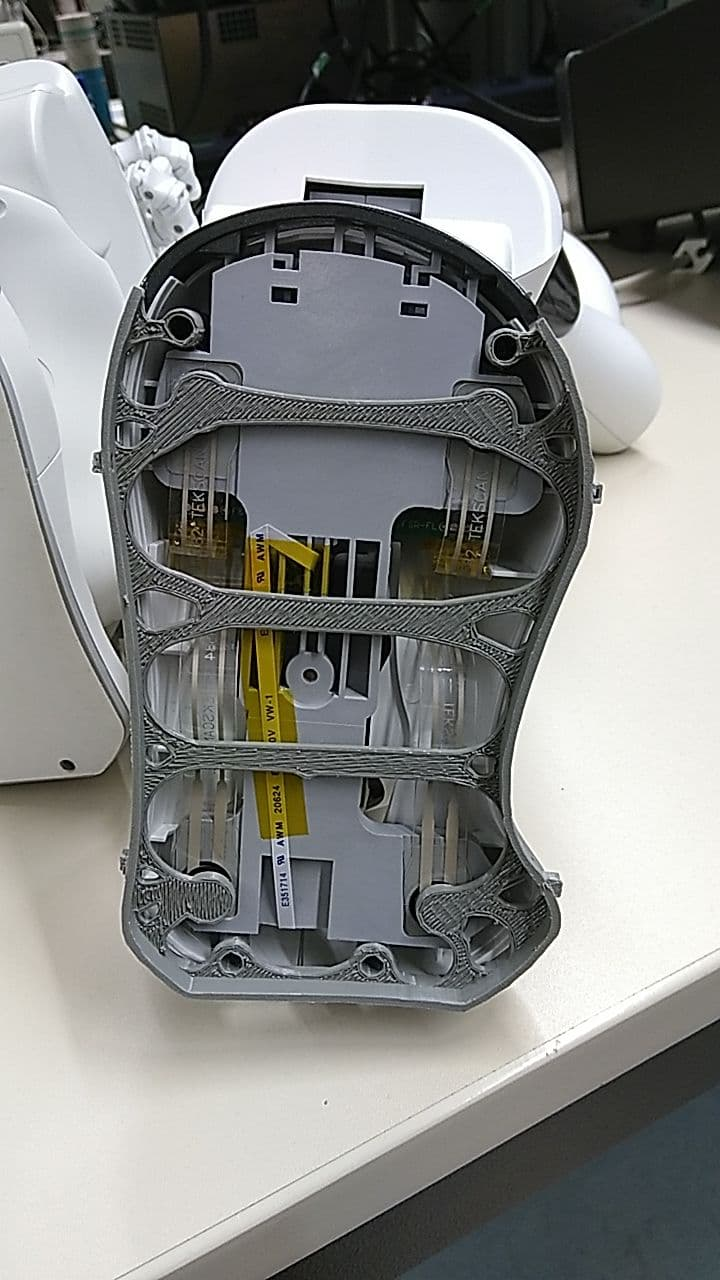
\includegraphics[width=\linewidth]{Bilder/Schuh_an_NAO_ohne_Sohle.jpg}
	\end{subfigure}
	\hfill
	\begin{subfigure}[c]{0.622\linewidth}
		\centering
		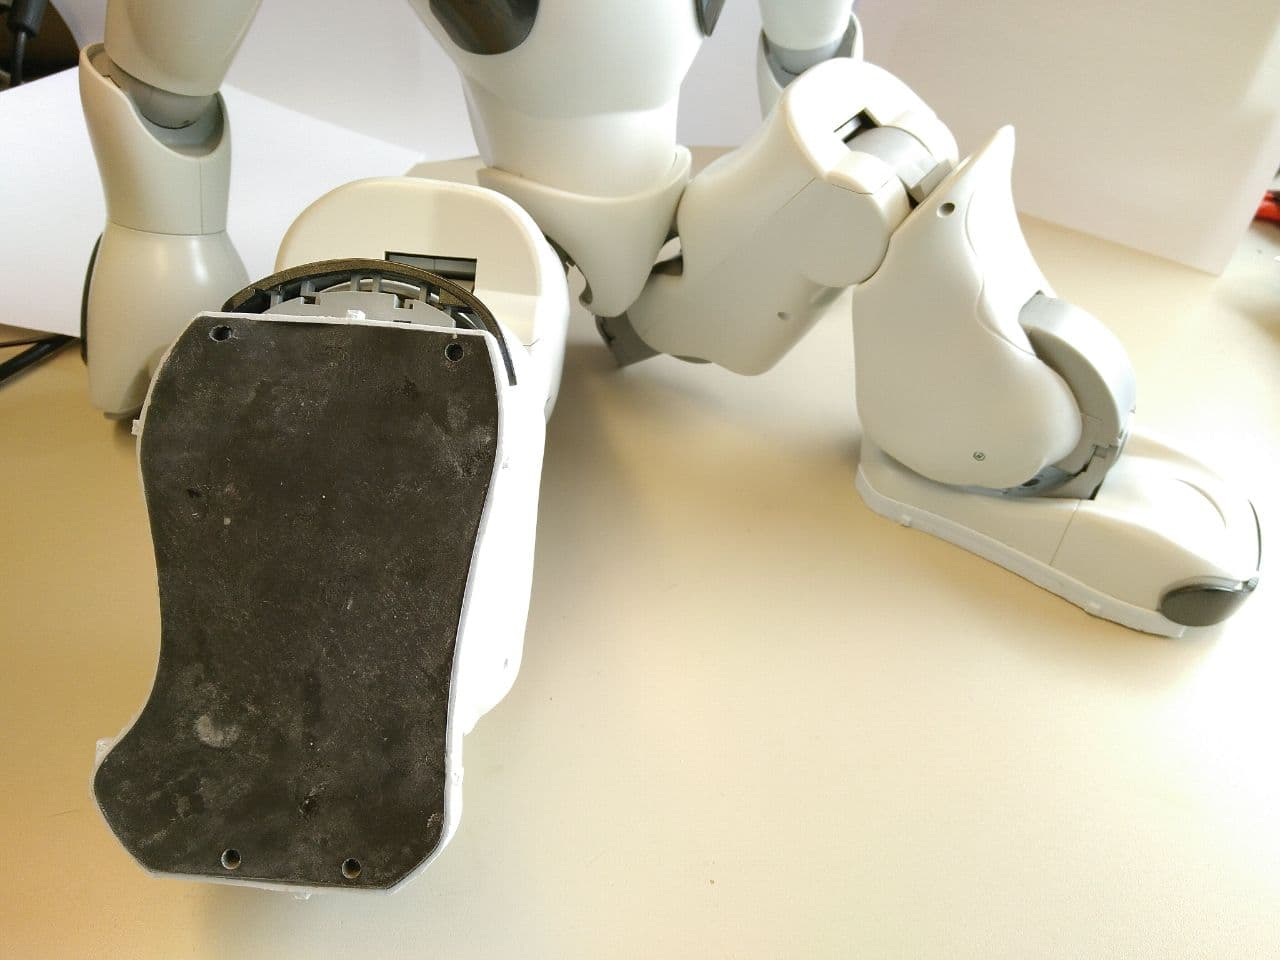
\includegraphics[width=\linewidth]{Bilder/Schuh_an_NAO_mit_Sohle.jpg}
	\end{subfigure}
	\hfill
	\caption{\textit{Links:} Der in Abb. \ref{Schuh_Inventor} in Autodesk Inventor erstellte Schuh aus PETG befestigt an der Unterseite des Fußes von NAO. \textit{Rechts:} Die aus der Gussform aus Abb. \ref{Gussform_Inventor} entnommene Sohle mit 20\,\% MAP Anteil befestigt in dem aus PETG gedruckten Schuh.}
	\label{nao_mit_schuhen}
\end{figure}

\begin{figure}[htb]
	\hfill
	\begin{subfigure}[c]{0.4\linewidth}
		\centering
		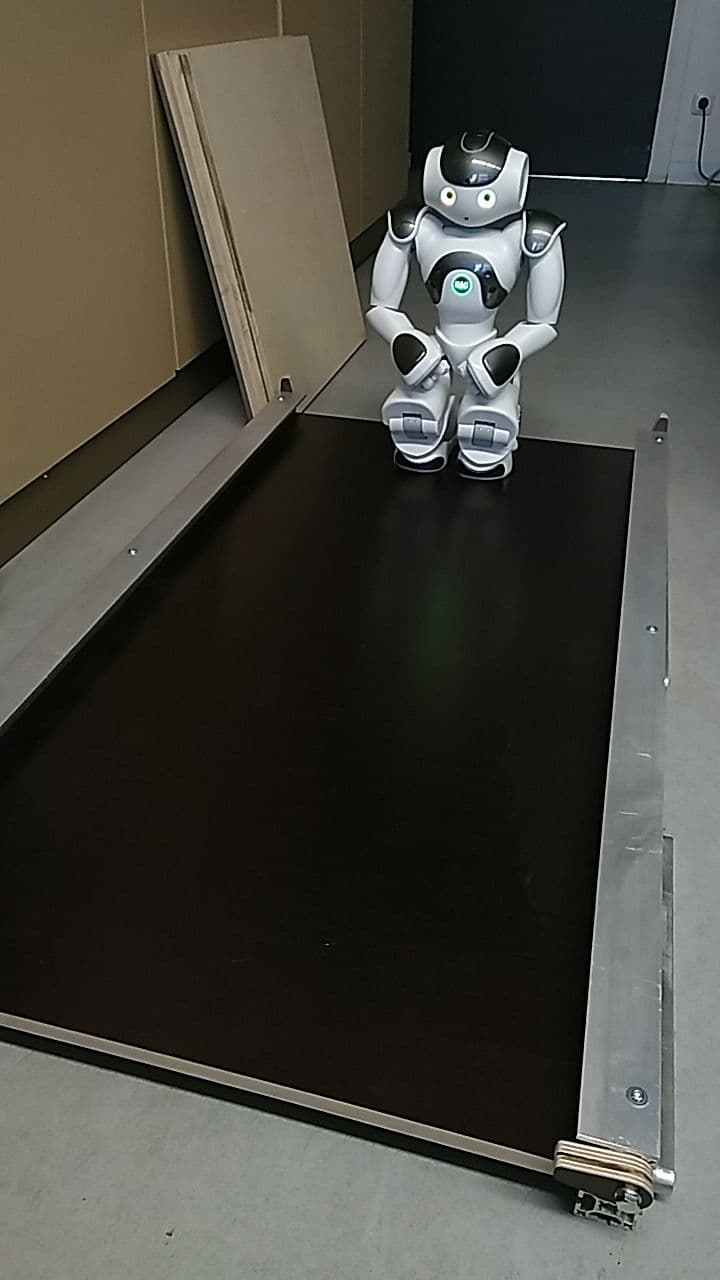
\includegraphics[width=\linewidth]{Bilder/NAO_auf_Rampe2.jpg}
	\end{subfigure}
	\hfill
	\begin{subfigure}[c]{0.4315\linewidth}
		\centering
		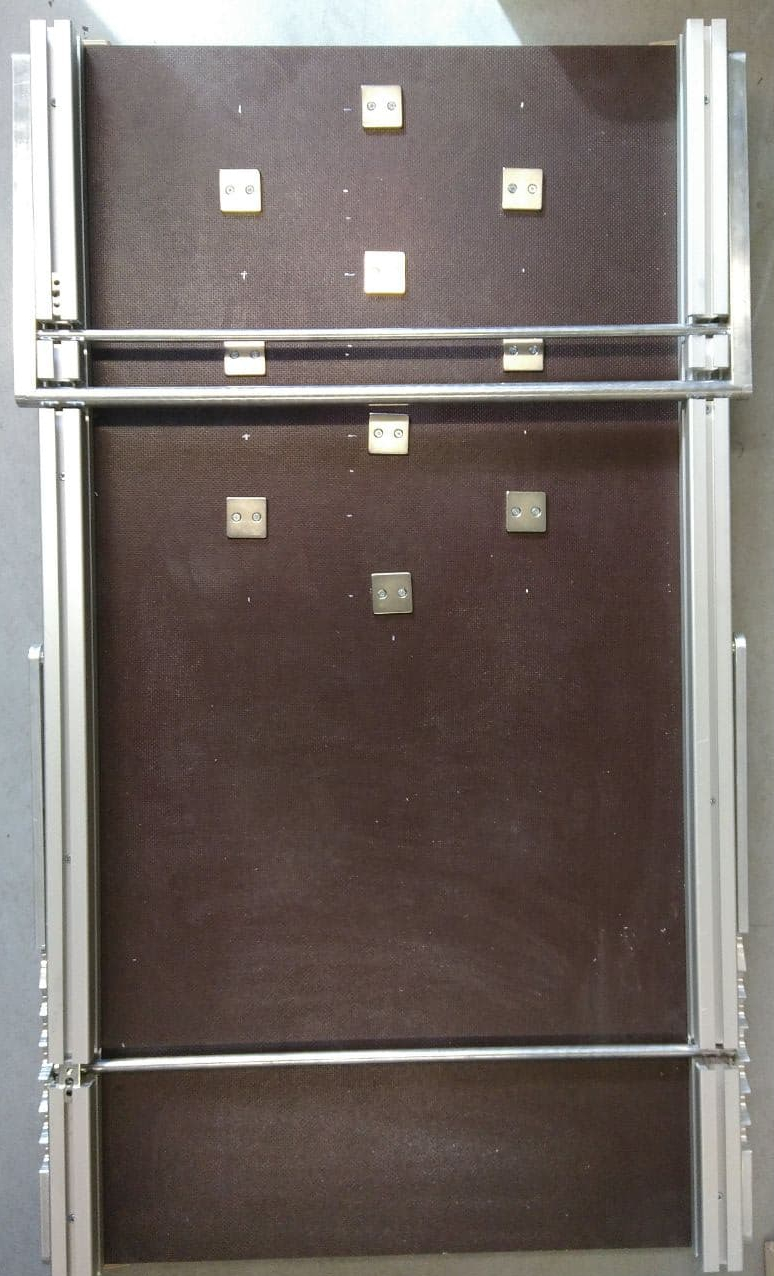
\includegraphics[width=\linewidth]{Bilder/magneten_an_rampe1_geschnitten.jpg}
	\end{subfigure}
	\hfill
	\caption{\textit{Links:} Der NAO Roboter steht im Ruhezustand an der Startposition auf der Rampe ohne Einlageplatten (an der Wand links neben NAO). \textit{Rechts:} Rampenunterseite mit befestigten Neodymmagneten.}
	\label{nao_und_rampe}
\end{figure}

Bereits in den vorherigen Kapiteln wurde auf die Durchführung dieses Versuchs eingegangen. Im Folgenden wird über den Ablauf und einige Problematiken gesprochen, welche sich während dem Herstellungs- und Laufprozess herauskristallisierten. 

Wie bereits in Kapitel \ref{Herstellung_MAP} beschrieben, wird zunächst das MAP hergestellt und anschließend in die Formen gegossen. Während der Vermengung wurde festgestellt, dass bei 60\,\%gem MAP die Durchmischung nicht gewährleistet werden kann, solang der verwendete Becher über die Hälfte voll ist. Deshalb wurden in diesem Fall zwei identische Proben hergestellt, welche erst in der Form zusammengegossen wurden. Alle anderen Proben mussten nach der Durchmischung in zwei separate Becher umverteilt werden, da während der Entgasung das Gemisch an Volumen bis zu einer Druckabnahme von etwa $15 \unit{mbar}$ zunimmt. Dies hat zur Folge, dass der Becher nur etwa halb voll sein darf, damit das MAP nicht \glqq überkocht\grqq{}. 

Nach spätestens 24 Stunden ist das Silikon vollständig ausgehärtet und kann aus der Form gelöst werden. Aufgrund der Einhängevorrichtung musste die Gussform hierbei aufgebrochen werden, um die nur $2 \unit{mm}$ dicken Stangen nicht abzubrechen oder aus dem MAP zu reißen. Zudem verkeilt sich das Silikon in den Unebenheiten des 3D Drucks, sodass selbst mithilfe von Silikonöl, welches vor dem Gießen in die Form gegeben werden kann, sich das MAP nur schwer lösen lässt. 

Um nun die Sohlen an dem Roboter anzubringen, wird zuerst der aus PETG bestehende Schuh angebracht, zu sehen in Abb. \ref{nao_mit_schuhen} links. Im Unterschied zu dem Originalteil ist dieser größtenteils offen und besitzt kein Gegenstück des Magneten unter der zweiten Strebe, welcher bei der Montage hilft. Anschließend wird die MAP Sohle durch Verbiegen und Druck eingehängt und schließt dadurch den Schuh ab, siehe Abb. \ref{nao_mit_schuhen} rechts. Nun ist der Roboter bereit für das Testen des Gangs.

Zunächst wurde der Laufsteg ohne Magneten verwendet. Erst nach der erfolgreichen Messung aller Sohlen, d.h. mit höchstens einem Sturz pro Messreihe, wurden die Magneten wie in Abb. \ref{nao_und_rampe} rechts zu sehen, angebracht. 

Zu Beginn jeder Messung wird NAO in hockender Position aufgestellt, Abb. \ref{nao_und_rampe} links. Dies ist seine Ruheposition, in der er gestartet wird und in die er bei dem Herunterfahren zurückkehrt. Der autonome Modus muss in Choregraphe (siehe Kapitel \ref{software}) bei Start ausgeschaltet werden, andernfalls würde NAO sich sofort aufstellen, sich leicht bewegen und bei Gesichtserkennung mit Spracherkennung beginnen und antworten. 

Sowohl über Lan als auch Wlan lässt sich über SSH eine Verbindung zu NAO herstellen. Um das Gleichgewicht besser messen zu können wurde Wlan genutzt. Über die Shell wurde das Programm \ref{Messungscode} (siehe Anhang) ausgeführt. Der Roboter steht zuerst auf, wobei seine Beine hierbei in einer schiebenden Bewegung zur Seite gedrückt werden. Dies hat zur Folge, dass bereits hier der Schuh zerstört wird, wenn die Sohlen nicht rutschen können. Anschließend wird die Messung begonnen während NAO den vorgefertigten Gang ausführt. 

Für jede Messabfrage benötigt der Roboter eine Verarbeitungszeit, das bedeutet, dass die Dauer eines Abfragendurchlaufs, also der Abfrage aller erwünschten Werte, an die Anzahl der Ausgaben gekoppelt ist. In den im folgenden Kapitel ausgewerteten Abfragen wurden insgesamt 24 unterschiedliche Sensorenausgaben eingeholt. Damit NAO hierbei etwa einen Meter Strecke zurücklegt, werden 220 Durchläufe dieser Abfragen durchgeführt (zu erkennen in der For-Schleife von Code \ref{Messungscode}). Schlussendlich nimmt NAO erneut die hockende Position ein und kann wieder an den Anfang des Laufstegs getragen werden. 

Anfangs war die Stabilität mit MAP Sohlen nicht gewährleistet. Dies lag zum einen daran, dass das Silikon am Boden durch Adhäsion festklebte. Dadurch wurde entweder die Sohle aus der Verankerung gerissen, NAO verlor das Gleichgewicht oder die Schuhe brachen. Dies wurde durch die bereits genannte Speisestärke verbessert. Ein weiteres Problem waren die Zylinder, welche den Schuh durch Schrauben an der Oberseite befestigen. Diese brachen meist auf Höhe der Querstreben, wodurch NAO sehr instabil wurde. Durch eine Verstärkung dieser Stellen in Autodesk konnte auch diese Schwachstelle eliminiert werden. 

\begin{wraptable}{r}{0.4\linewidth}
	\vspace{-0.8cm}
	\caption{Gemessenes Gewicht des Originalschuhs und des Ersatzes zur Verwendung von MAP als Laufuntergrund.}\label{gewicht}
	\begin{tabular}{ll}\\\toprule  
		Gewogenenes Bauteil & Gewicht \\\midrule
		Originalschuhteil & $61 \unit{g}$ \\  \midrule
		PETG Schuhgerüst &$16 \unit{g}$ \\  \midrule
		MAP mit 20\% CIP &$88 \unit{g}$ \\  \midrule
		MAP mit 40\% CIP &$107,5 \unit{g}$ \\  \midrule
		Sohle mit 60\% MAP &$182 \unit{g}$ \\  \bottomrule
	\end{tabular}
    \vspace{-2cm}
\end{wraptable} 

Die Schräglagefunktion der Rampe wurde nicht genutzt. Grund hierfür ist eine sehr differenzierte Herangehensweise des Gangs, die erforderlich wäre, damit NAO laufen kann, siehe auch \cite{Lutz_naowalking}.

Zur besseren Vergleichbarkeit wurden schließlich die Sohle von NAO und alle angebrachten Teile gewogen. Hierbei ergab sich, dass die Originalsohle um über $30\unit{g}$ leichter ist, als der leichteste Schuh, zu sehen in Tabelle \ref{gewicht}. Ein höherer CIP Anteil hat nicht nur zur Folge, dass das MAP an Festigkeit zunimmt, sondern trägt auch erheblich zu dem Gesamtgewicht bei. 


